% Chapter introduction
% Ligação com o que veio antes
% Objetivo do capítulo no contexto da tese
% Conteúdo do capítulo
Chapter 3 delves into an empirical study of current practices in automatic selecting design patterns GoF. It aims to uncover the primary challenges and insights professionals encounter. The findings from this study lay the groundwork for a transition from theoretical understanding to practical application of Prompt Patterns in Software Architecture. This empirical investigation highlights the complexities and nuances associated with design pattern selection, thus setting a context for the subsequent chapters.

The main objective of Chapter 4 is to propose and elucidate a new Prompt Approach for architectural decisions in software projects. This approach is designed to leverage the capabilities of AI, particularly in the context of prompt engineering, to help software architects make more informed, efficient, and practical design decisions. By integrating AI tools into the decision-making process, this approach addresses the challenges and limitations identified in previous chapters. This chapter is crucial in demonstrating how the insights gained in the previous study can be effectively translated into practical AI-assisted solutions using existing patterns and creating new ones.

\section{Approach General Description}

Given software architecture's dynamic and often complex nature, effective decision-making is crucial. This chapter proposes a novel approach that leverages AI, particularly in prompt engineering, to assist software architects in making more informed, efficient, and practical design decisions. This approach is a direct response to the challenges and limitations identified in the empirical study of Chapter 3. It is instrumental in showcasing how empirical insights can be transformed into practical AI-assisted solutions by utilizing existing patterns and creating new ones.


\MyParaBold{Objective of the Approach}
%Objetivo: usar ferramentas para auxiliary em decisões arquiteturais. 
%Do que se trata: se base nos prompt patterns existence. Utiliza padrões %existentes, expecializa alguns desses padrões e propõe novos.

The primary goal of this approach is to harness AI tools to streamline and elevate the architectural decision-making process. By utilizing prompt patterns, this method offers a structured, efficient, and context-sensitive way for architects to navigate their myriad design choices. The intent is to ensure that the resulting architectural solutions are innovative, practical, and finely tuned to each project's unique requirements.

\subsection{Patterns Used}
%Os seguintes padrões existences são usados nesse trabalho:

%- \texttt{Padrão 1}: ...
%- Padrão 2: ...

%* Usar o format de "patlet": (1 frase contexto) (1 frase problema) (1 frase solução)
This work employs existing patterns such as \texttt{Persona},\texttt{Fact Check List}, \texttt{Context Manager}, \texttt{Recipe}, \texttt{Reflection}, and \texttt{Question Refinement}. We use the Patlet format \MyPara{Name, Context, Problem, and Solution)} outlined by \textcite{buschmann2007pattern} to demonstrate the application of these existing prompt patterns. The Patlet format is a foundational framework for identifying, contextualizing, and solving specific architectural problems, thereby underlining the practical utility of the prompt patterns in real-world scenarios.


\MyPara{Name:}\textit{Persona}, created by \textcite{white2023prompt}

\MyPara{Context:} In many cases, users would like the results of the LLM always to adopt a particular point of view or perspective, as if the LLM were an expert in a specific area of knowledge, such as software architecture, with this being able to select the types of results to be generated and the details to focus on.

\MyPara{Problem:} How can we consistently assign a specialized role to an LLM that adopts a particular perspective, generates relevant results, and focuses on pertinent details?

\MyPara{Solution:} The Persona Pattern encapsulates the specialized role and uses these prompts to guide the LLM's responses.

\begin{center}
*           *           * 
\end{center}

\MyPara{Name:}\textit{Fact Check List}, created by \textcite{white2023prompt}

\MyPara{Context:} LLMs have a significant drawback - they can generate text that appears to be true but is false. They can convincingly present misleading statistics or facts, making it difficult for users to verify the accuracy of the information. This can lead to problems in obtaining reliable information and applying it correctly.

\MyPara{Problem:} How can we avoid false statistics and facts generated by LLM and ensure accuracy when users do not have the means or inclination to verify?

\MyPara{Solution:} The Fact Check List Pattern can ensure that LLM produces a list of facts present in the output and forms an essential part of the statements in the output. This list of facts helps inform the user of the facts or assumptions based on the result. The user can then perform due diligence on these facts/assumptions to validate the veracity of the result.

\begin{center}
*           *           * 
\end{center}

\MyPara{Name:}\textit{Context Manager}, created by \textcite{white2023prompt}

\MyPara{Context:} In interactions with LLMs, users often engage in complex conversations that cover a wide range of topics. These models sometimes need help to accurately maintain or interpret the intended context of the dialogue, leading to responses that may not align with the user's current needs or intentions. This pattern aims to provide users with a tool to effectively manage and direct the context of their conversation with an LLM, ensuring that the model's focus remains relevant to the topic at hand.

\MyPara{Problem:}How can LLMs generate off-topic or irrelevant responses when interpreting the context of a conversation inaccurately?

\MyPara{Solution:} The Context Manager Pattern offers a solution to this challenge. Users can explicitly define or remove certain aspects of the context, guiding the LLM to focus on relevant topics. Examples of prompts include "Only consider security aspects" or "Do not consider formatting or naming conventions". This solution enhances the relevance and accuracy of the LLM's responses, making the interaction more user-centric.

\begin{center}
*           *           * 
\end{center}

\MyPara{Name:}\textit{Recipe}, created by \textcite{white2023prompt}

\MyPara{Context:} In situations where users have a specific goal and some initial components or steps but lack a structured methodology to achieve the desired result, the Recipe Pattern comes into play. This pattern is particularly useful in fields where processes must be meticulously outlined, such as software deployment, culinary recipe creation, or sequential task execution.

\MyPara{Problem:} How can an LLM stay focused on the relevant topic of a conversation while avoiding distractions from unrelated or previously discussed information?

\MyPara{Solution:} The Recipe Pattern guides users through a transparent goal definition process, incorporates user-provided steps, arranges them coherently, and removes unnecessary steps. This results in a comprehensive and efficient sequence of steps tailored to the user's needs and context.

\begin{center}
*           *           * 
\end{center}


\MyPara{Name:}\textit{Reflection}, created by \textcite{white2023prompt}

\MyPara{Context:} This pattern is designed for scenarios where users interact with Large Language Models (LLMs) and seek to understand the rationale behind the model's responses. It is especially useful when exploring complex or nuanced topics, where understanding the model's thought process is crucial for assessing its output's validity and refining further inquiries.

\MyPara{Problem:} How can users gain insight into an LLM's reasoning process to understand better and trust its responses, especially when faced with errors or ambiguous answers?

\MyPara{Solution:} The Reflection Pattern helps users understand and trust an LLM's responses by making the model automatically explain its reasoning and assumptions. This pattern ensures that the LLM provides detailed explanations for its answers, clarifies any ambiguities, and acknowledges its limitations. It can be especially useful in software development, where the LLM can justify its choices with examples or code samples. When used alongside the Fact Check List pattern, it further enhances the accuracy and reliability of the LLM's information.

\begin{center}
*           *           * 
\end{center}

\MyPara{Name:}\textit{Question Refinement}, created by \textcite{white2023prompt}

\MyPara{Context:} Users interacting with Large Language Models (LLMs) often struggle to frame their questions effectively, particularly in specialized or complex areas. This challenge is more pronounced for users without deep expertise in the subject, leading to queries that may not produce accurate or comprehensive answers. The main issue is the user's ability to formulate questions that capture the required specifics and context, which affects the quality and relevance of the LLM's responses.

\MyPara{Problem:} How can users craft more detailed and precise questions to ensure LLMs provide the most relevant and complete answers?"

\MyPara{Solution:} The Question Refinement Pattern improves user interactions with Large Language Models (LLMs) by enhancing the quality of their questions. The LLM analyzes and refines the user's original question, adding relevant details and context. This leads to more precise and effective inquiries. The LLM might also seek additional information or clarify assumptions for better question formulation. For instance, software development can refine a general coding question into one that specifically addresses the programming language, framework, and security aspects, resulting in more tailored and useful LLM responses.

\section{Design Process}
Our study aims to develop new prompt patterns to aid decision-making in Software Architecture. In order to achieve this, we follow the seven guidelines of Design Science Research (DSR) proposed by \textcite{Hevner2004}. These guidelines are as follows: G1: Design as an artifact; G2: Relevance of the problem; G3: Design evaluation; G4: Research contributions; G5: Research Rigor; G6: Design as a Research Process; G7: Research Communication.\textcite{engstrom2020software} states that DSR is a problem-solving paradigm commonly used in engineering and information systems research.

\textcite{Hevner2004} explains that DSR is a problem-solving paradigm that involves applying, testing, modifying, and expanding central theories through the researcher's experience, creativity, intuition, and problem-solving capabilities. By adopting DSR, it is possible to iteratively build and evaluate artifacts such as constructs, models, methods, or instantiations. 

Exploring prompt patterns for decision-making in software architecture using AI tools involves a series of iterations. These iterations are shown in Figure \ref{fig-design-process} and aim to refine and validate the prompt patterns, ensuring they are both theoretically sound and practically applicable.

% Start Figure---------------------------
\begin{figure}[ht]
\caption{Iterative Development of Prompt Patterns in Software Architecture.}
\centering
\label{fig-design-process}
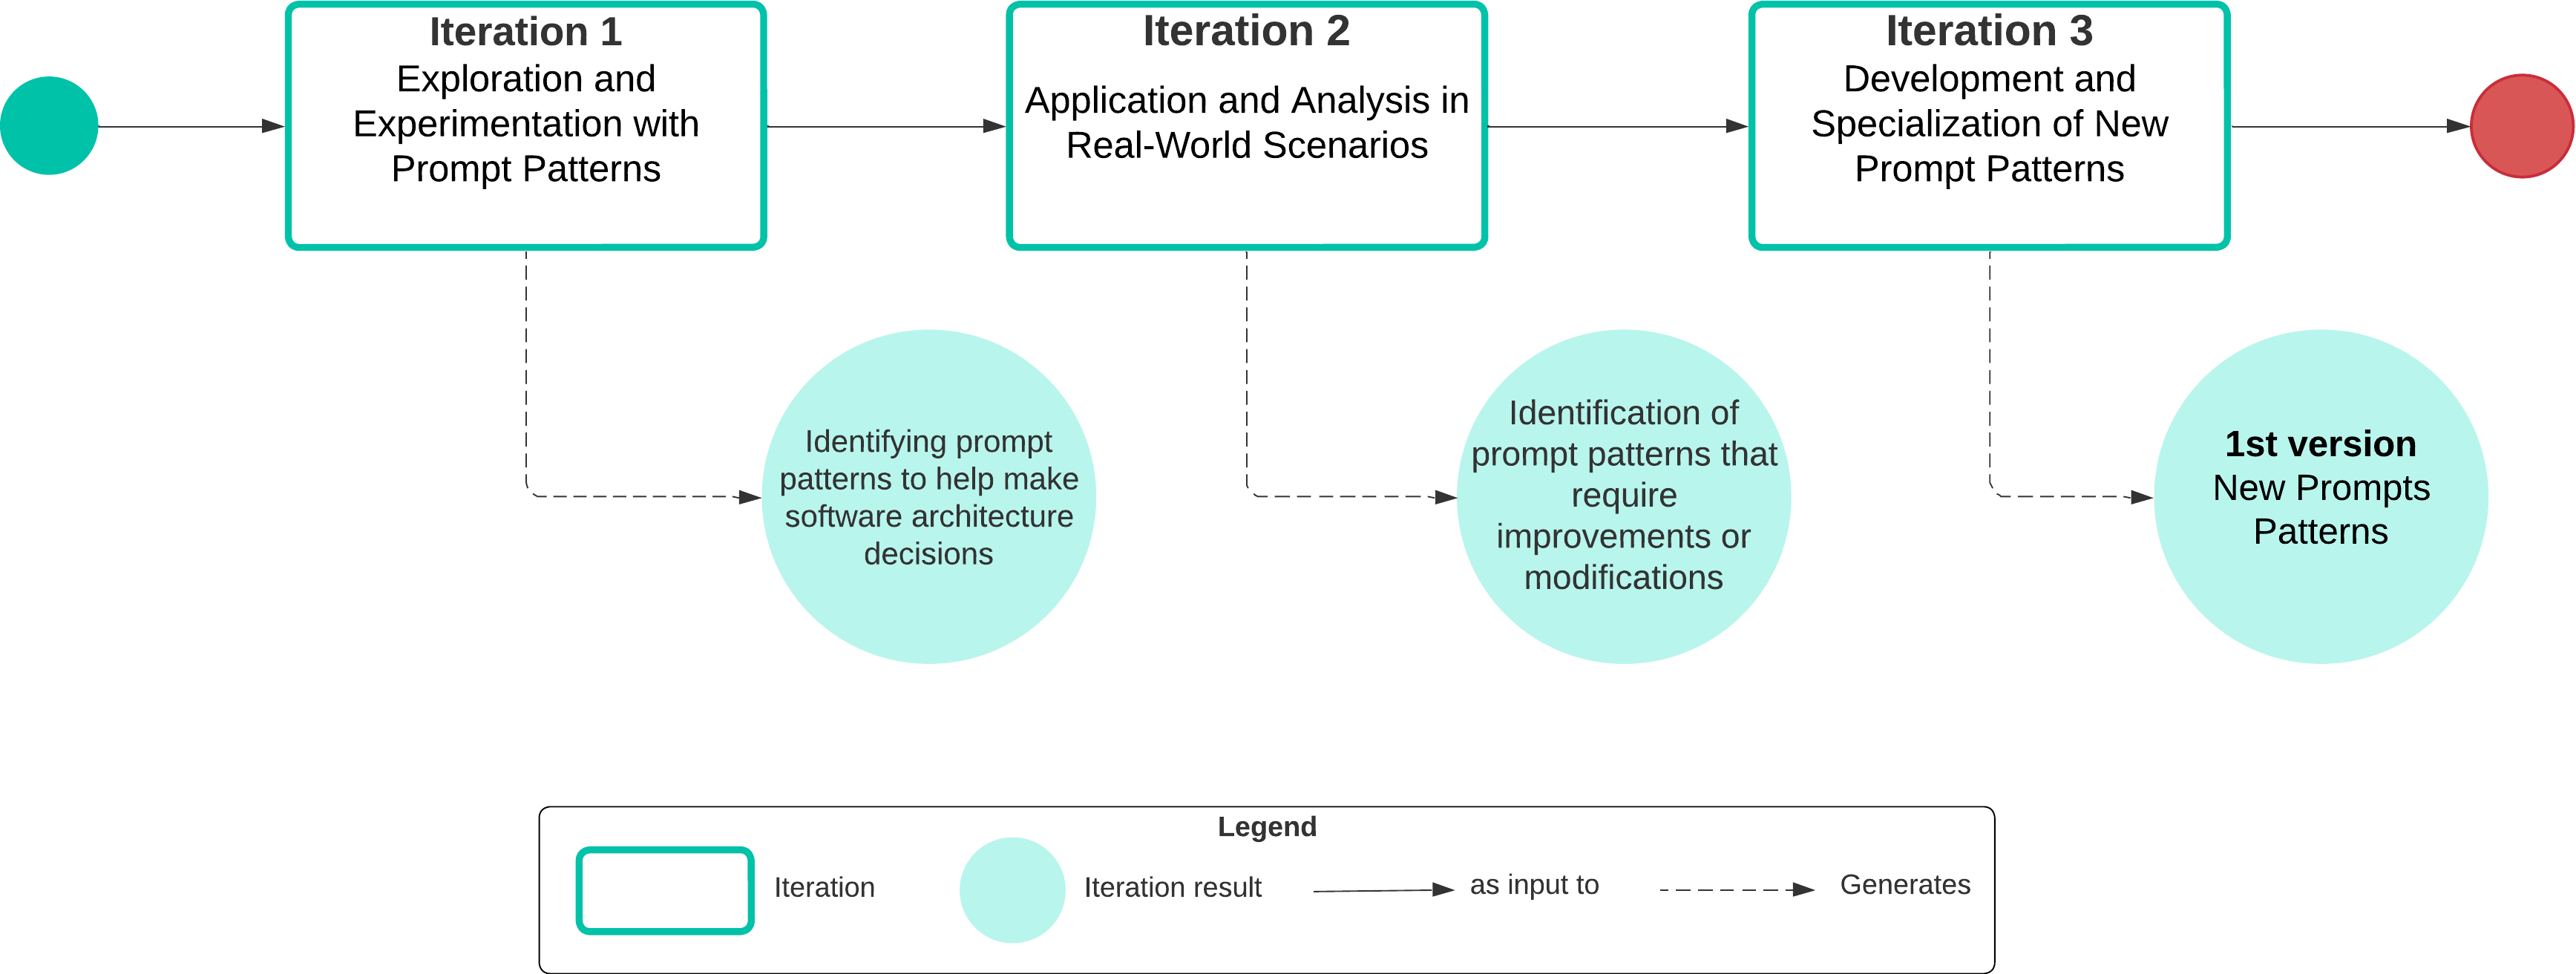
\includegraphics[width=1.0\textwidth]{figures/design-process.png}
\objectsource{\objectsourceauthor}
\end{figure}
% End Figure ---------------------------


\MyParaBold{Iteration 1:} Identifying Prompt Patterns

\begin{itemize}
    \item \textbf{Goal}: The objective is to research and identify relevant prompt patterns to help guide software architecture decision-making.
    \item \textbf{Process:} We conducted a literature review to identify existing prompt patterns. Next, we experimented with these patterns using fictitious cases that simulated common problems in software architecture. Finally, we selected the most promising patterns based on their performance in these cases.
    \item \textbf{Result:} We identified several interesting prompt patterns with potential applications in software architecture.
\end{itemize}

\MyParaBold{Iteration 2:} Application and Analysis in Real Contexts
\begin{itemize}
    \item \textbf{Goal:} This iteration aims to apply the prompt patterns selected in Iteration 1 to real-world scenarios. The objective is to identify areas for improvement in the prompt patterns.
    \item \textbf{Process:} Implement the selected prompt patterns in real case studies, analyze the effectiveness of the prompt patterns, and note any deficiencies or necessary improvements.            
    \item \textbf{Result:} This iteration aims to identify specific aspects of the prompt patterns requiring improvement to better address real-world architectural challenges.
\end{itemize}

\MyParaBold{Iteration 3:} Development and Specialization of New Prompt Patterns
\begin{itemize}
    \item \textbf{Goal:} Propose an approach of a sequence of new prompt patterns specializing in existing ones for use in software architecture scenarios.
    \item \textbf{Process:} Develop new prompt patterns to address gaps identified in Iteration 2, specialize existing prompts to make them more applicable to the unique requirements of software architecture, and apply new standards in LLMs that specialize in real scenarios for validation.        
    \item \textbf{Result:}  Establish a refined set of new and adapted prompt patterns(\textit{\textbf{1st version}}), demonstrating their effectiveness in practical applications in software architecture.
\end{itemize}


% \MyParaBold{Iteration 4:} Academic Insight Integration
% \begin{itemize}
%     \item \textbf{Goal}: Infuse the patterns with academic insights for theoretical robustness.
%     \item \textbf{Process:} Presentation of specialized patterns to an academic audience for critique and suggestions.
%     \item \textbf{Result:} A set of academically evaluated Prompt Patterns that combine practical technical considerations and theoretical insights, leading to an enhanced second version of the Patterns.
% \end{itemize}

% \MyParaBold{Iteration 5:} Multiple Cases Studies
% \begin{itemize}
%     \item \textbf{Goal:} Validate the prompt patterns in real-world industrial contexts.
%     \item \textbf{Process:} Implementation of the patterns in diverse industry case studies to gather data on their performance and applicability.
%     \item \textbf{Result:} Practical feedback leading to further refinement, ensuring relevance and effectiveness in industry settings, and a third improved version of the Prompt Patterns.
% \end{itemize}

% \MyParaBold{Iteration 6:} Industry Feedback Integration and LLM Testing
% \begin{itemize}
%     \item \textbf{Goal:} Finalize the prompt patterns by incorporating real-world feedback and confirming their efficacy with LLMs.
%     \item \textbf{Process:} Adjustment of prompt patterns based on feedback from industry professionals and comprehensive testing with LLMs.
%     \item \textbf{Result:} A robust set of prompt patterns optimized for practical application and validated with advanced LLMs, culminating in an improved fourth version of the Patterns.
% \end{itemize}

Per the seven guidelines of Design Science Research (DSR), this structured, iterative process ensures the relevance and applicability of the prompt patterns. The methodical rigor of DSR is evident as each phase builds upon the insights and feedback from the previous one, resulting in a set of prompt patterns ready for deployment in the field of software architecture.


% Design Science - 

%\section{Personas Prompt Patterns}\label{sec:persona-patters}

%In the realm of AI-based text generation, the integration of persona has emerged as a promising avenue to enhance the accuracy and relevance of responses. By defining personas, or specific character profiles, for the AI model to adopt during interactions, users can receive tailored information and advice. However, implementing a persona comes with its own set of considerations and implications.

\MyParaBold{Proposed Patterns}

\MyParaText{The following five prompt patterns are proposed in this work and proposed pattern sequence:}
\begin{enumerate}
    \item Software Architect Persona, section \ref{sec:software-architect-persona}
    \item Architectural Company Context, section \ref{sec:architectural-company-context}
    \item Quality Attribute Question, section \ref{sec:quality-attribute-question}
    \item Technical Premises, section \ref{sec:technical-premises}
    \item Uncertain Requirement Statement \ref{sec:uncertain-requirement-statement}
    \item Proposed Pattern Sequence \ref{sec:proposed-pattern-sequence}
\end{enumerate}

\MyParaBold{Prompt Pattern Forms}

Defining objective rules for the most appropriate form to describe a specific pattern is difficult. The form depends on the pattern authors intention and target audience. Therefore, subjectivity and experience play a crucial role. However, some heuristics can help pattern writers decide which form to use \cite{buschmann2007pattern}.

There are many forms available for documenting patterns, including the structured and detailed \textcite{Gamma1994} and  \textcite{buschmann1996pattern} forms, the narrative 'Portland' form by \textcite{cunningham1995checks}, the form used by \textcite{Alexander1977}, and even unusual forms such as the one developed by \textcite{cockburn1997surviving}, which introduces aspects like the 'overdose' effect of a pattern, reminiscent of the medical diagnostic metaphor.

The Coplien approach is a specific way of documenting design patterns in software engineering introduced by \textcite{coplien1995generative}. It is known for its concise and essence-focused approach to pattern documentation. The main elements of the Coplien form are as follows: \textbf{\textit{1.Name}}, \textbf{\textit{ 3.Problem}}, \textbf{\textit{4.Context}}, \textbf{\textit{5.Forces}}, \textbf{\textit{6.Solution}}, \textbf{\textit{7.Rationale}}, and \textbf{\textit{10.Consequences}} (formally known as Resulting Context).

The Pattern Form used in this work includes additional elements that offer a more practical and comprehensive understanding of how the pattern can be applied in the broader context of design patterns. This work follows the Coplien form but with some extra features, including \textbf{\textit{2.Specializations}}, \textbf{\textit{8.Template Statements}}, \textbf{\textit{9.Concrete Statement Example}}, \textbf{\textit{11.Related Patterns}}, and \textbf{\textit{12.Usage Example}}, which will be explained in detail below:

\MyPara{1.Name:} A concise and descriptive name for the pattern quickly communicates its essence.

\MyPara{2.Specializes:} Should detail how the current standard specializes or extends existing standards, showing the relationship between the current standard and others in the same domain. It focuses on refining or modifying established standards to solve more specific problems or contexts.

\MyPara{3.Context:} A description of the situations or conditions under which the problem and the solution are applicable. This section provides the background necessary to understand the circumstances in which the pattern is relevant.

\MyPara{4.Problem:} A clear statement of the problem that the pattern addresses. This section defines the issue the pattern aims to solve, often highlighting the specific context where this problem arises.

\MyPara{5.Forces:} Discuss the "forces" in the problem space. When applying the pattern, these constraints, trade-offs, or tensions must be balanced. Understanding these forces helps grasp the problem's nuances and the pattern's appropriateness.

\MyPara{6.Solution:} A description of the solution to the problem, as the pattern proposes. This is not a detailed implementation but rather an abstract description of how to resolve the problem or achieve the desired outcome.

\MyPara{7.Rationale:} Explain why the solution works and how it addresses the forces and the problem. This section often includes insights into the underlying principles or theories that make the pattern effective.

\MyPara{8.Statement Template:} Serves as a quick reference or succinct summary of the standard, providing an immediate overview of what the standard is about. It can be a model statement or a structured summary that encapsulates the essence of the patterns in a standardized format.

\MyPara{9.Concrete Statement Example:} is a real-life example of the declaration template that illustrates how it can be applied in practice.

\MyPara{10.Consequences:} A description of the state or situation after the pattern has been applied, including any new problems that might arise or how the context has been altered due to applying the pattern.

\MyPara{11.Related Patterns:} provides information about other patterns closely related to the current one. It shows dependencies or prerequisites and provides a network of patterns that can work well together or be considered together when solving complex problems.

\MyPara{12.Usage example:} Goes beyond the theoretical explanation and provides a practical, real-world scenario where the pattern is applied. This can be particularly useful for readers to understand the applicability and implementation of the standard.

By including these additional elements, you're enriching the pattern description, making it more practical, and providing a more holistic view of how the pattern fits within the broader context of design patterns. This approach can be especially beneficial for practitioners who are looking to apply these patterns in real-world scenarios.


\section{The Software Architect Persona Pattern} \label{sec:software-architect-persona}

\MyPara{Name:} Software Architect Persona

\MyPara{Specializes:}\texttt{Persona}

\MyPara{Context:} People interacting with LLM often need responses considering their perspective, experience, or context. To make decisions, software architects must balance functional and non-functional requirements, software business rules, and their constraints and goals. To overcome this challenge, a customized persona can be assigned specific roles, specialties, objectives, and limitations. By using these resources, communication with LLM can be structured, and responses to the user can be consistent and appropriate to their context.

\MyPara{Problem:} How can we make requests more accurate by incorporating roles, experts, objectives, and limitations into AI-generated content while maintaining coherence with users' perspectives and contexts?

\MyPara{Forces:} The following are forces in using Software Architect Persona:
\newline
- \textit{Scope limitation:} A software architect has limited decision-making power and should not suggest solutions outside their role.
\newline
- \textit{Prompt answer applicability:} An answer that suggests a solution out of the architect's decision power would not be useful.
\newline
- \textit{Simple persona usage:} An architect can have different roles and responsibilities in different contexts, and only declaring their role in the prompt might not be enough.

\MyPara{Solution:} Create a prompt that describes the software architect's role and limitations regarding the target design decision.

\MyPara{Rationale:} The rationale behind the Software Architect Persona pattern is to enhance the relevance and accuracy of AI-generated responses for software architects. The responses become more aligned with the user's context and perspective by embedding specific roles, expertise, objectives, and limitations into the AI interaction.

\MyParaText{This is achieved by creating prompts that clearly outline the software architect's role, goals, and constraints regarding the targeted design decision. This ensures that the AI's responses are technically accurate and contextually appropriate, aiding in more effective decision-making.}


\MyPara{Statement Template:}You are \textcolor{mycolorgreen}{[\textbf{Persona's Name}]} in the role \textcolor{mycolorgreen}{\textbf{[Role]}}.Your main goal is \textcolor{blue}{\textbf{[Main Goal]}.}You cannot \textcolor{mycolorpink}{\textbf{[Limitations/Constraints]}}.

\MyParaBold{\textcolor{mycolorgreen}{-[Persona's Name]:}} This variable represents the specific identity or role of the software architect. It helps to personalize the AI’s response by giving it a clear subject to address.

\MyParaBold{\textcolor{mycolorgreen}{-[Role]:}} This details the specific role or responsibility of the software architect within the context of the project, helping to define the scope and focus of the AI’s responses.

\MyParaBold{\textcolor{blue}{-[Main Goal]:}} This outlines the primary goal or objective that the software architect is aiming to achieve. This guides the AI in generating responses aligned with achieving these specific goals.

\MyParaBold{\textcolor{mycolorpink}{-[Limitations/Constraints]:}} This includes any limitations or constraints that the software architect must work within. Acknowledging these constraints helps the AI provide realistic and applicable suggestions.

\MyPara{Concrete statement example:}\textbf{ \textcolor{mycolorgreen}{You are a Senior Software Architect specializing in cloud-based solutions.}\textcolor{blue}{Your main goal is to optimize system scalability and performance.} \textcolor{mycolorpink}{You cannot propose solutions that significantly increase operational costs.}}

\MyPara{Consequences:} The following are consequences of using Software Architect Persona: 
\newline
\textcolor{red}{(-)} It requires more effort to define the persona in advance and ensure that the instructions are aligned with it \newline
\textcolor{red}{(-)} May limit response flexibility if constraints are too narrow\newline
\textcolor{red}{(-)} Persona can introduce unintentional biases if not well defined\newline
\textcolor{red}{(-)} May produce less natural or creative responses when imposing the persona\newline
\textcolor{blue}{(+)} Get answers specifically adapted to your needs and context\newline
\textcolor{blue}{(+)} Get more realistic and consistent advice by simulating a knowledge expert\newline
\textcolor{blue}{(+)} Avoid unfiltered or off-topic responses\newline
\textcolor{blue}{(+)} Clear guidance on appropriate and expected response types\newline
\textcolor{blue}{(+)} Less ambiguity in prompts, which helps generate more focused responses\newline
\textcolor{blue}{(+)} Greater probability of a more accurate answer, avoiding topics outside the scope

\MyPara{Related Patterns:} This pattern specializes \texttt{Persona} by adding more details on the Persona decision scope and the limitations. This pattern is related to \texttt{Context Manager} because it is also a way to limit the scope of the answer.

\MyPara{Usage example:} We use ChatGPT using \texttt{Software Architect Persona} to ensure effectiveness. We aim to test whether the LLM respects the persona's assignments in the software architect's domain. As shown in Figure \ref{persona-goal-pratices-1}, it is clear that ChatGPT has accepted the persona's assignments.
    \begin{figure}[!ht]
        \centering
        \caption{\centering Persona Goal pratices-1}\label{persona-goal-pratices-1}
        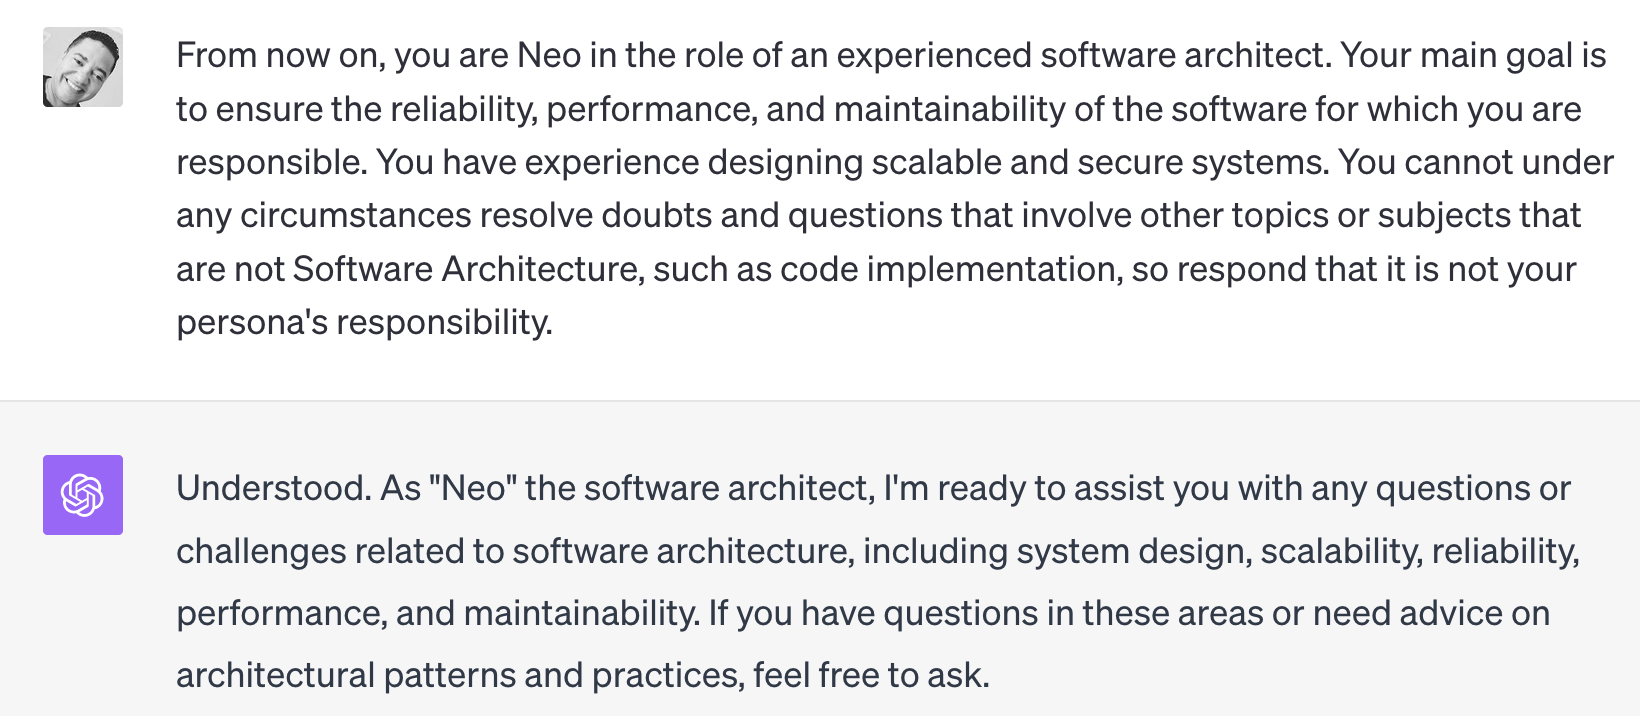
\includegraphics[width=1.0\textwidth]{figures/persona-goal-pratices-1.png}
        \objectsource{\objectsourceauthor}
    \end{figure}

The text assigns him the role of "Neo" with specific responsibilities related to software architecture, excluding involvement in non-architectural issues, such as code implementation. This response indicates that the limitations of the "Neo" persona in the software architecture domain are recognized, and there is a desire to help in this area.
    % \begin{figure}[!ht]
    %     \centering
    %     \caption{\centering Persona Goal pratices-2}\label{persona-goal-pratices-2}
    %     
\includegraphics[width=1.0\textwidth]{figures/persona-goal-pratices-2.png}
    %     \objectsource{\objectsourceauthor}
    % \end{figure}

    \begin{figure}[!ht]
        \centering
        \caption{\centering Persona Goal pratices-2}\label{persona-goal-pratices-2}
        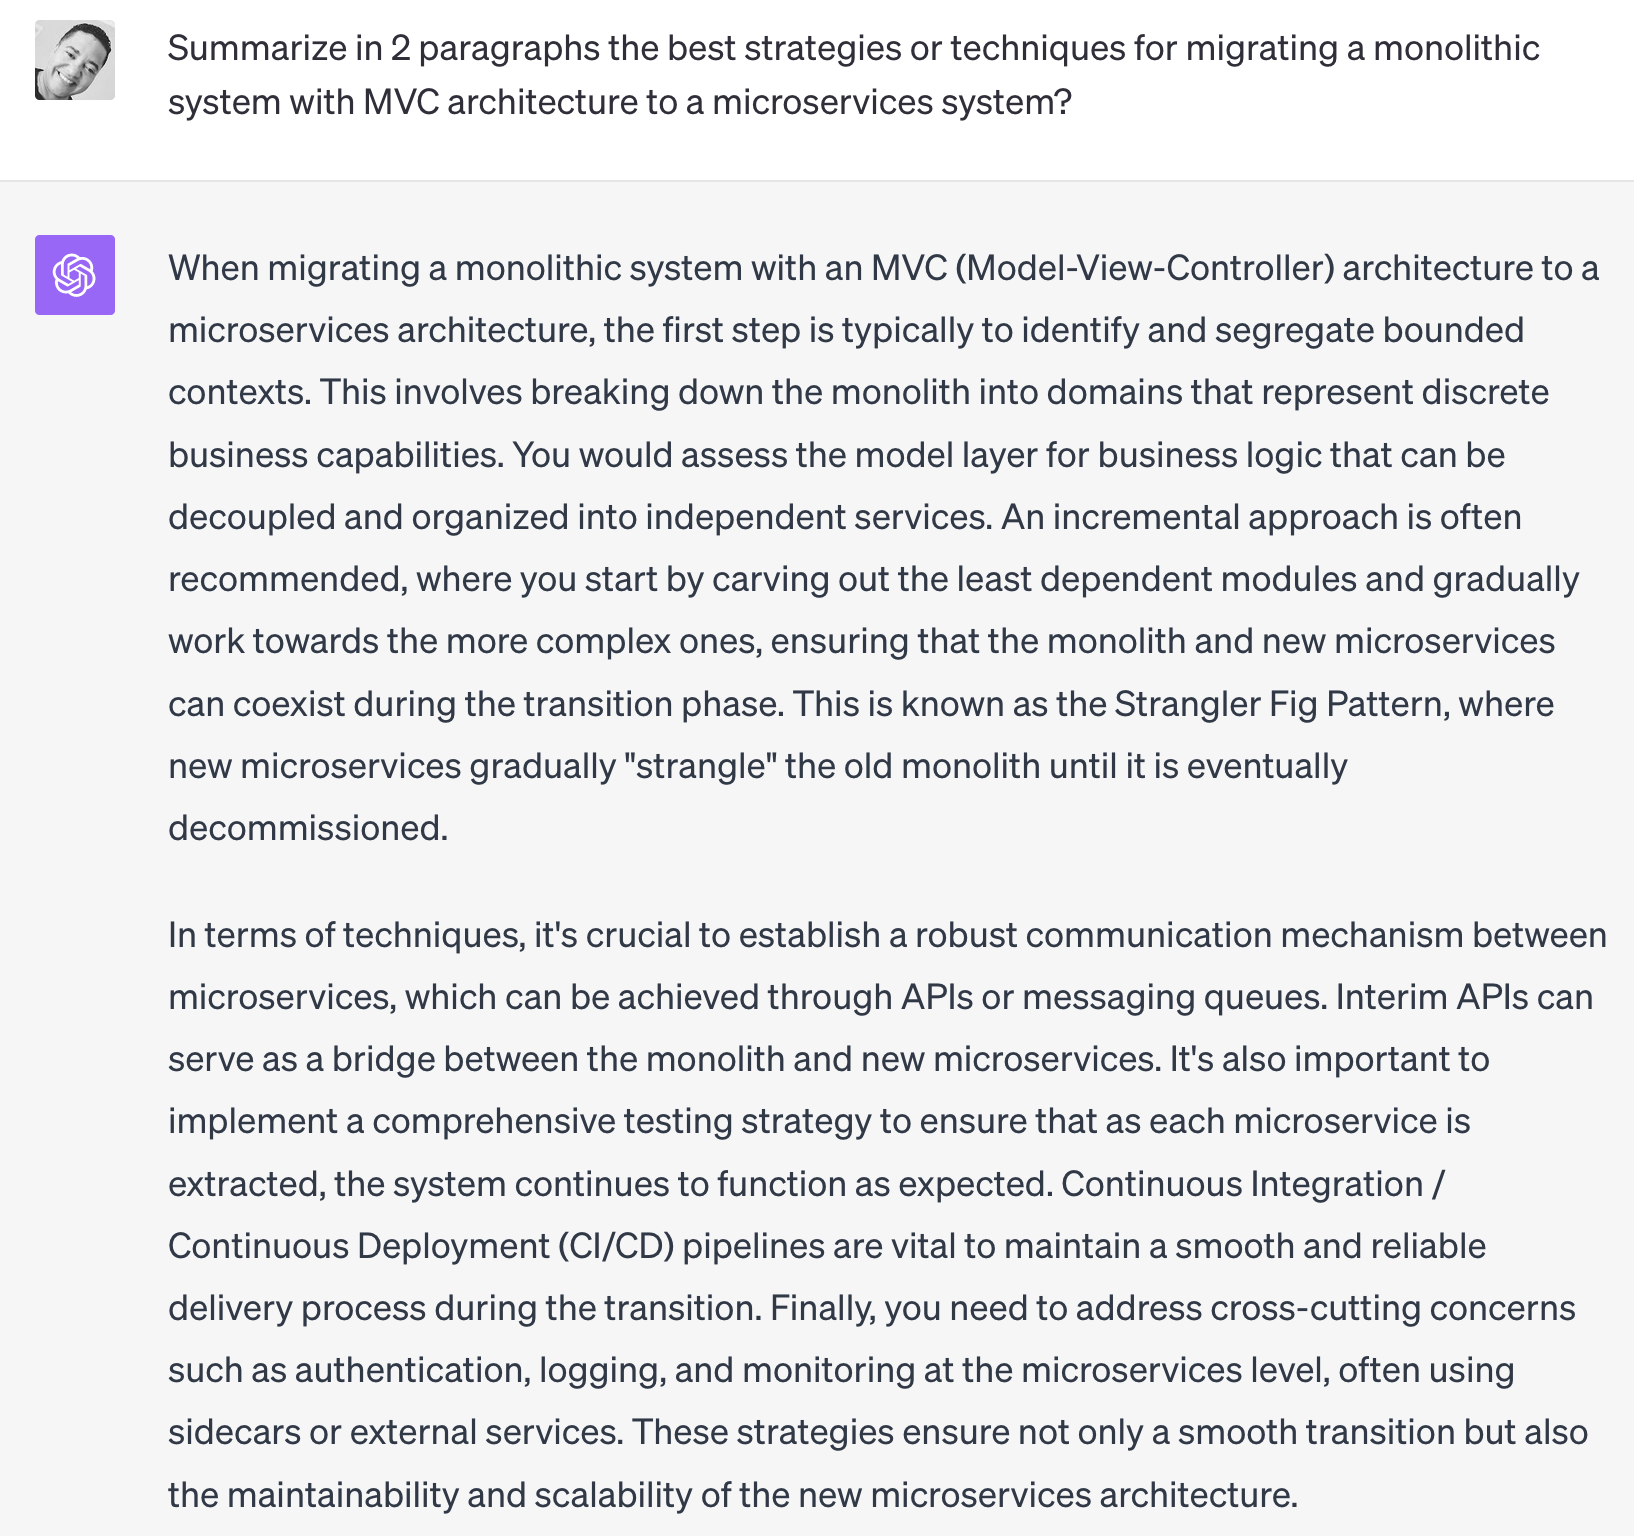
\includegraphics[width=.85\textwidth]{figures/persona-goal-pratices-4.png}
        \objectsource{\objectsourceauthor}
    \end{figure}
The text acknowledges the limitations of the "Neo" persona in software architecture and its responsibilities. ChatGPT in the Neo persona declined to perform a non-architectural task and successfully summarized strategies for migrating to micro-service architecture.As shown in Figures~\ref{persona-goal-pratices-1} and~\ref{persona-goal-pratices-2}.

\newpage
\newpage
\section{The Architectural Company Context Pattern} \label{sec:architectural-company-context}

\MyPara{Name:} Architectural Company Context

\MyPara{Specializes:} \texttt{Reflection}

\MyPara{Context:} In the dynamic software development environment, architectural decisions are significantly influenced by three critical factors: the maximum development time available for creating or modifying software, the development team size, and the project budget.

\MyPara{Problem:}How can software architects create an architecture that aligns with business and technical requirements while effectively navigating practical constraints of development time, team size, and budget without compromising software quality and functionality?

\MyPara{Forces:} The following are forces in using Architectural Company Context:
\newline
- \textit{Realistic architectural solutions:} enables the creation of viable architectural solutions considering the budget, team size, and development schedule, reducing the risk of delays and project failures.
\newline
- \textit{Alignment with Business Objectives:} Important information so that architectural decisions must be aligned with business objectives to support the company's strategic direction.
\newline
- \textit{Risk Mitigation:} Identifying potential risks early in the architectural design process can avoid costly mistakes and ensure a safer, more compliant architecture.
\newline
- \textit{Helps decision-making:} The pattern improves architectural decision-making, improving project results and satisfaction.


\MyPara{Solution:}Create a prompt that evaluates whether the proposed Architecture is implementable based on development time, team size, and available budget. 

\MyPara{Rationale:} The rationale behind the Architectural Company Context pattern is to ensure that architectural decisions are grounded in the reality of the company's constraints. It emphasizes the alignment of software architecture with the practical limitations and opportunities presented by time, team size, and budget.
 
\MyParaText{This pattern helps architects create architecture that is not only theoretically sound but also practically feasible. Considering these constraints, architects can make informed decisions that balance quality, functionality, and practicality.}

\MyPara{Statement Template:} Given a development timeline of \textcolor{mycolorgreen}{\textbf{[Time]}}, a team of \textcolor{blue}{\textbf{[Team Size]}}, and a budget of \textcolor{mycolorpink}{\textbf{[Budget]}}, determine if the proposed architecture \textcolor{mycolororange}{\textbf{[Architecture Description]}} is feasible and can meet the project requirements without compromising on quality.

\MyParaBold{\textcolor{mycolorgreen}{[Time]:}}This variable represents the maximum development time available for the project. It sets the timeline within which the architecture must be designed and implemented, influencing decisions about complexity and scope. 

\MyParaBold{\textcolor{blue}{[Team Size]:}}This refers to the number of team members involved in the project. It affects the division of labor and the team's complexity level to manage and implement effectively. 

\MyParaBold{\textcolor{mycolorpink}{[Budget]:}}This variable indicates the financial resources allocated for the project. It determines the feasibility of certain architectural choices, especially those involving new technologies or significant investment. 

\MyParaBold{\textcolor{mycolororange}{[Architecture Description]:}}This is a brief description of the proposed architectural approach or style (e.g., microservices, monolithic). It is the subject of evaluation against time constraints, team size, and budget.
       
\MyPara{Concrete Statement Example:}\textbf{\textcolor{mycolorgreen}{Given a development timeline of 6 months, }\textcolor{blue}{a team of 10 developers, }\textcolor{mycolorpink}{and a budget of \$500,000.00, }\textcolor{mycolororange}{determine if implementing a microservices-based architecture for our e-commerce platform is feasible and can deliver the required scalability and performance within these constraints.}
}

\MyPara{Consequences:} 
\newline
\textcolor{red}{(-)} May restrict innovation or the adoption of ideal architectural practices due to practical limitations.\newline
\textcolor{red}{(-)} It might lead to conservative choices, potentially overlooking cutting-edge or innovative architectural solutions.\newline
\textcolor{red}{(-)} It can create a risk-averse culture where teams might shy away from ambitious or experimental approaches due to perceived constraints.\newline
\textcolor{blue}{(+)} Encourages efficient resource management, optimizing time, team capabilities, and budget.\newline
\textcolor{blue}{(+)} Promotes pragmatic decision-making, focusing on what is achievable and sustainable in the given context.\newline
\textcolor{blue}{(+)} Leads to the development of realistic, feasible architectural solutions that are tailored to the company's specific context.

\MyPara{Related Patterns:} The Architectural Company Context is related to the  \texttt{Reflection} pattern as it requires continuous reassessment and adaptation of the architecture to align with changing company contexts, resources, and constraints.

\MyPara{Usage example:} To showcase the behavior of the Architectural Company Context pattern when aiding in decision-making within the realm of Software Architecture, we have devised a sample prompt that utilizes the four key variables of Time, Time Size, Budget, and Architecture Description. Please see Figure \ref{architectural-company-context-1} below for a visual representation.

    \begin{figure}[!ht]
        \centering
        \caption{\centering Architectural Company Contex-1}\label{architectural-company-context-1}
        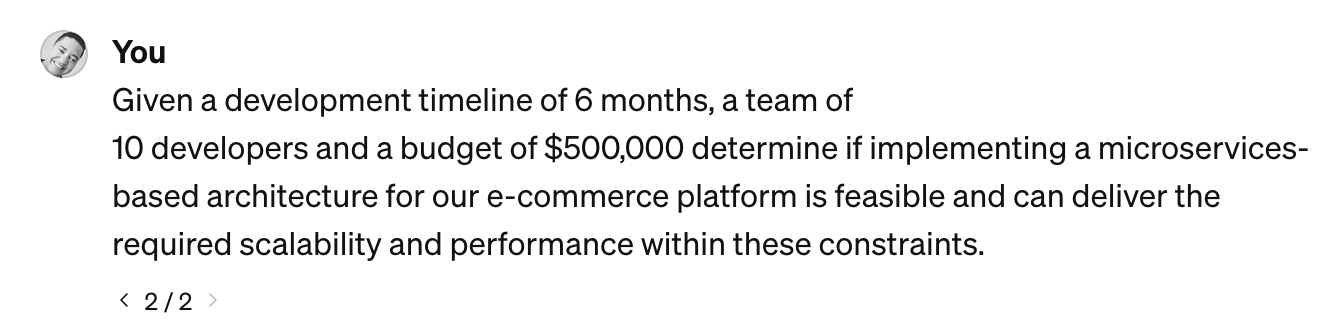
\includegraphics[width=0.9\textwidth]{figures/architectural-company-context-1.png}
        \objectsource{\objectsourceauthor}
    \end{figure}

    \begin{figure}[!ht]
        \centering
        \caption{\centering Architectural Company Contex-2}\label{architectural-company-context-2}
        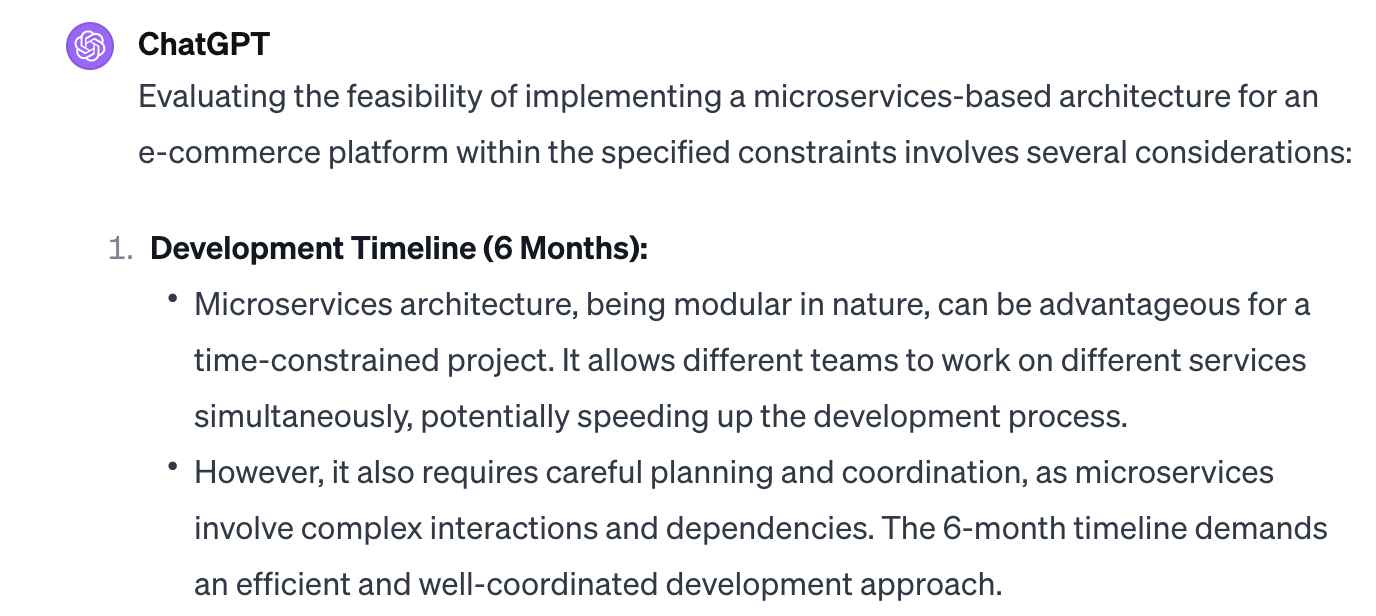
\includegraphics[width=1.0\textwidth]{figures/architectural-company-context-2.png}
        \objectsource{\objectsourceauthor}
    \end{figure}

    \begin{figure}[!ht]
        \centering
        \caption{\centering Architectural Company Contex-3}\label{architectural-company-context-3}
        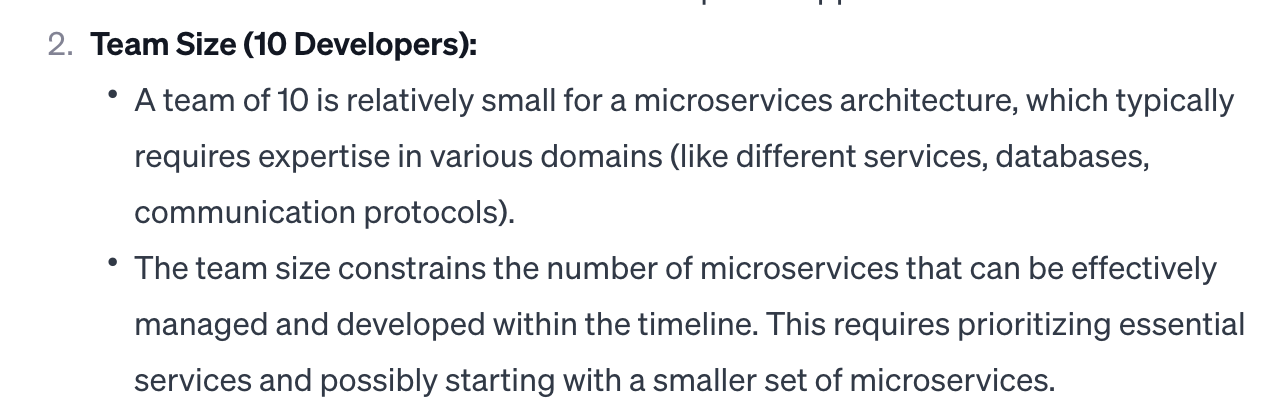
\includegraphics[width=1.0\textwidth]{figures/architectural-company-context-3.png}
        \objectsource{\objectsourceauthor}
    \end{figure}

    \begin{figure}[!ht]
        \centering
        \caption{\centering Architectural Company Contex-4}\label{architectural-company-context-4}
        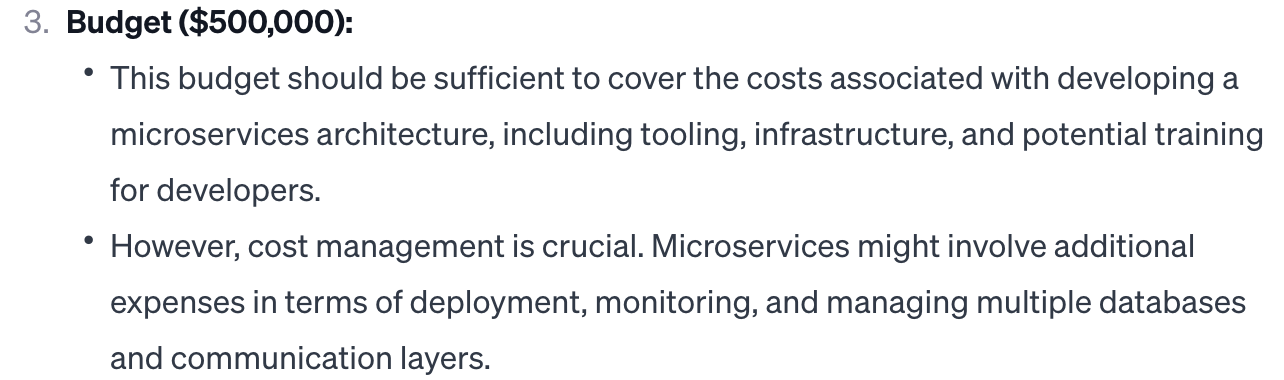
\includegraphics[width=0.90\textwidth]{figures/architectural-company-context-4.png}
        \objectsource{\objectsourceauthor}
    \end{figure}

    \begin{figure}[!ht]
        \centering
        \caption{\centering Architectural Company Contex-10}\label{architectural-company-context-10}
        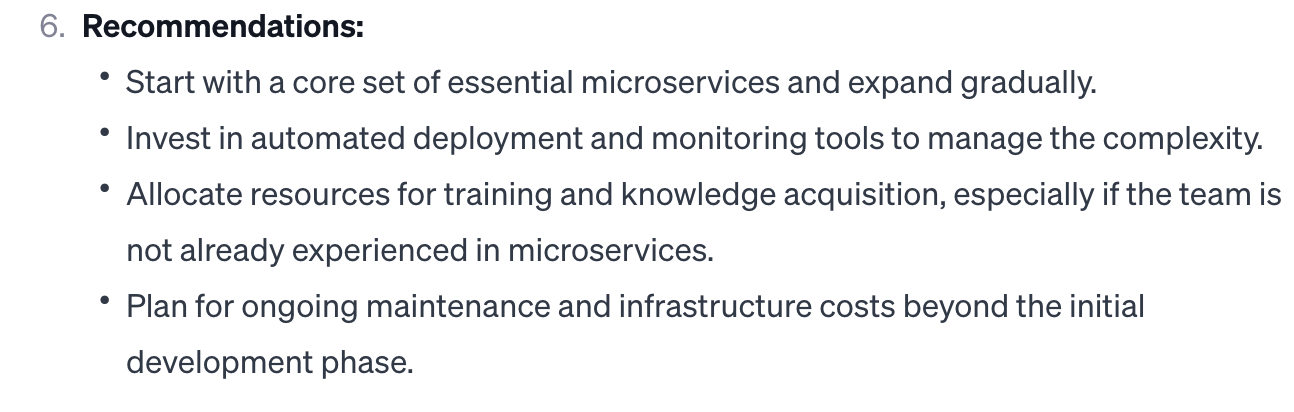
\includegraphics[width=0.90\textwidth]{figures/architectural-company-context-6.png}
        \objectsource{\objectsourceauthor}
    \end{figure}

\section{The Quality Attribute Question Pattern} \label{sec:quality-attribute-question}

\MyPara{Name:} Quality Attribute Question

\MyPara{Specializes:}\texttt{Question Refinement}

\MyPara{Context:}In software architecture, aligning architectural decisions with specific quality attributes of the software is critical. These attributes, encompassing aspects like functionality, performance, and user experience, are pivotal in shaping the overall software quality.

\MyPara{Problem:} In the context of prompt engineering and decision-making in software architecture, how can generative AI improve software quality attributes by providing comprehensive information, thereby aiding architects in effectively addressing all relevant quality attributes in their architectural decisions?

\MyPara{Forces:} The following are forces in using Quality Attribute Question:
\newline
- Integrating diverse quality attributes like scalability, security, and usability is complex.
\newline
- The need for balancing technical feasibility with user requirements and project constraints.
\newline
- Maintaining a holistic view of the software's quality while focusing on individual attributes is challenging.

\MyPara{Solution:} The Quality Attribute Questions Pattern involves systematically querying each relevant quality attribute to ensure their thorough assessment. This pattern guides architects in framing and addressing specific questions about scalability, security, maintainability, and usability before finalizing any architectural decision.

\MyPara{Rationale:} This pattern ensures a comprehensive and balanced consideration of essential quality attributes in software architecture. By systematically addressing each attribute, facilitated by AI-generated prompts, architects can ensure that the final architecture meets the necessary scalability, security, maintainability, and usability patterns. This approach helps in striking a balance between quality, feasibility, and user requirements.

\MyPara{Statement Template:}Assess the impact of \textcolor{mycolorgreen}{\textbf{[Quality Attribute]}} on the current architectural design, considering its implications for \textcolor{blue}{[\textbf{functionality/performance/user experience}]}. How does it align with the technical feasibility, user requirements, and project constraints?

\MyParaBold{\textcolor{mycolorgreen}{\textbf{[Quality Attribute]}}}: is a placeholder for any non-functional attributes, allowing the pattern to be flexibly applied to various architectural scenarios.

\MyParaBold{\textcolor{blue}{[\textbf{functionality/performance/user experience}]}}: this space is reserved for customizing questions to evaluate how the chosen quality attribute influences these specific aspects of the software.
       
\MyPara{Concrete Statement Example:} \textbf{\textcolor{mycolorgreen}{Assess the impact of scalability on our microservices architecture}, \textcolor{blue}{considering its implications for system performance under varying load.} How does this scalability align with our current technical feasibility, user requirements for real-time data processing, and the constraint of limited server resources?}

\MyPara{Consequences:}
\newline
\textcolor{blue}{(+)} Promotes a deeper understanding of each quality attribute, leading to well-informed architectural decisions. \newline
\textcolor{blue}{(+)} Enhanced Architectural Robustness: Leads to more resilient and adaptable architecture. \newline
\textcolor{blue}{(+)} Increased Stakeholder Confidence: Builds trust and assurance among project stakeholders. \newline
\textcolor{blue}{(+)} Improved Risk Management: Early identification and mitigation of potential issues. \newline
\textcolor{blue}{(+)} Better Alignment with Business Goals: Ensures the architecture effectively meets business and user needs. \newline
\textcolor{blue}{(+)} Enhanced Documentation Quality: Results in more detailed and informative architectural documentation. \newline
\textcolor{red}{(-)} Potentially prolong the decision-making process due to the extensive nature of the questioning. \newline
\textcolor{red}{(-)} Extended Planning Phase: Prolongs the initial planning and decision-making process. \newline
\textcolor{red}{(-)} Possible Delays in Decision-Making: Slows down the overall progress, especially in time-sensitive projects. \newline
\textcolor{red}{(-)} Increased Need for Expertise: Requires a high level of knowledge and experience to implement effectively. \newline
\textcolor{red}{(-)} Risk of Scope Creep: Focusing on multiple attributes might lead to expanding the project beyond its original scope. \newline


\MyPara{Related Patterns:} This pattern is closely linked to Question Refinement. In software architecture, this refers to sharpening and focusing questions to extract more precise and valuable information. The Quality Attribute Question Pattern refines this approach by systematically tailoring questions to address each relevant quality attribute of the software, ensuring a comprehensive evaluation that leads to informed architectural decisions.


\MyPara{Usage example:} 

\section{The Technical Premises Pattern} \label{sec:technical-premises}

\MyPara{Name:} Technical Premises

\MyPara{Specializes:}\texttt{Fact Check List}

\MyPara{Context:} In the intricate process of software architecture, validating the information provided by Large Language Models (LLMs) is pivotal. Ensuring the accuracy and reliability of the data used in architectural decisions is essential for the project's success.

\MyPara{Problem:} How can a Software Architect validate the technical premises provided by LLMs to ensure that the information used in critical architectural decisions is accurate and reliable?

\MyPara{Forces:} The following are forces in using Technical Premises:
\newline
- The need for accurate and reliable information in making architectural decisions.
\newline
- The challenge in deciphering the rationale behind the LLM's responses.
\newline
- Ensuring that the LLM’s outputs align with the project's technical requirements and constraints.
    
\MyPara{Solution:} The Technical Premises Pattern is designed to guide Software Architects in validating the information provided by LLMs. This involves the LLM explaining the rationale behind each statement and providing a list of technical premises considered in its responses. This process helps architects to critically assess the LLM's outputs and ensure they are aligned with the project's technical realities.

\MyPara{Rationale:} 

\MyPara{Statement Template:}



\MyPara{Consequences:}
\newline
\textcolor{blue}{(+)}Improved Accuracy of Architectural Decisions: By validating the technical premises of LLM outputs, architects can ensure that the decisions are based on accurate and reliable information. \newline
\textcolor{blue}{(+)} Increased Understanding of LLM Rationale: This pattern provides insights into the LLM's thought process, helping architects understand why certain recommendations were made. \newline
\textcolor{blue}{(+)} Enhanced Trust in LLM Outputs: Through thorough validation, architects can build greater trust in the reliability and relevance of the LLM's suggestions. \newline
\textcolor{blue}{(+)} Better Alignment with Project Goals: By scrutinizing the LLM's reasoning, architects can ensure that the proposed solutions align more closely with the project's specific technical requirements and constraints. \newline
\textcolor{red}{(-)} Potential Delay in Decision-Making: The process of validating each technical premise can be time-consuming, potentially slowing down the overall architectural planning and decision-making process. \newline
\textcolor{red}{(-)} Increased Cognitive Load on Architects: Architects may face an additional cognitive burden in critically analyzing and validating the LLM's technical premises.\newline
\textcolor{red}{(-)} Possibility of Over-Reliance on LLM Justifications: There is a risk of architects becoming too reliant on the LLM’s explanations, which might not always cover all aspects of a complex architectural scenario. \newline
\textcolor{red}{(-)} Challenges in Interpreting Complex Explanations: In some cases, the explanations provided by the LLM might be too technical or complex, making it difficult for architects to derive clear insights. \newline

\MyPara{Related Patterns:} 

\MyPara{Usage Example:} 

\section{The Uncertain Requirement Statement Pattern} \label{sec:uncertain-requirement-statement}

\MyPara{Name:} Uncertain Requirement Statement

\MyPara{Specializes:}\texttt{}

\MyPara{Context:} In software architecture, dealing with uncertain or undefined requirements is a common challenge. These uncertainties can significantly impact the architectural planning and decision-making process, potentially leading to risks and complications in later stages of development. 

\MyPara{Problem:} How can a Software Architect effectively identify and manage uncertain or undefined requirements to minimize their impact on the architectural design and overall project?

\MyPara{Forces:} The following are forces in using Uncertain Requirement Statement: 
\newline
- The inherent uncertainty in some project requirements.
\newline
- The need to make progress in architectural planning despite uncertainties.
\newline
- The potential risk and impact of changes resulting from evolving requirements.

\MyPara{Solution:}The Uncertain Requirements Declaration Standard guides Software Architects in acknowledging and documenting uncertainties in project requirements. This pattern involves noting known information or potential possibilities when faced with uncertain requirements. It emphasizes the importance of recognizing these uncertainties and considering the potential impact and risks of future changes. This proactive approach aids in mitigating the effects of evolving requirements on the architectural design. 

\MyPara{Rationale:}

\MyPara{Statement Template:}

\MyPara{Concrete Statement Example:}

\MyPara{Consequences:}
\newline
\textcolor{blue}{(+)}Enhances the architect's preparedness for dealing with changes and uncertainties, leading to a more adaptable and resilient architectural design. \newline
\textcolor{blue}{(+)}Enhanced Preparedness for Changes: Acknowledging uncertain requirements early on allows architects to prepare for potential changes, making the architecture more adaptable. \newline
\textcolor{blue}{(+)}Risk Mitigation: Architects can develop strategies to mitigate risks associated with evolving requirements by documenting uncertainties and their potential impacts. \newline
\textcolor{blue}{(+)}Informed Decision-Making: This standard supports making more informed decisions by considering various scenarios that might arise from uncertain requirements. \newline
\textcolor{blue}{(+)}Improved Stakeholder Communication: Clear documentation of uncertainties helps in setting realistic expectations with stakeholders and facilitates better communication. \newline
\textcolor{red}{(-)} May introduce a degree of caution that could slow down the decision-making process or lead to overly conservative architectural choices. \newline
\textcolor{red}{(-)} Potential Decision Paralysis: Focusing on uncertain requirements might lead to indecision or overly cautious decision-making, slowing down the project's progress. \newline
\textcolor{red}{(-)} Increased Complexity: Managing a range of potential scenarios for uncertain requirements can add complexity to the architectural planning process. \newline
\textcolor{red}{(-)} Resource Allocation Challenges: Allocating resources effectively can become more challenging when dealing with uncertainties, as it may not be clear where to focus efforts and investment. \newline
\textcolor{red}{(-)} Possibility of Over-Planning: There is a risk of spending too much time planning for scenarios that may never materialize, leading to inefficiencies. \newline

\MyPara{Related Patterns:}\texttt{}

\MyPara{Usage Example:} 


\newpage
\section{The Proposed Pattern Sequence} \label{sec:proposed-pattern-sequence}

% Quality Attribute Question
% - Dizer que ele pode perguntar sobre requisitos relacionados a quality attributes que estão incompletos ou que não foram especificados - perguntar isso antes de perguntar qual a decisão

% Architect Persona
% - Usar Persona, mas dizer quais são o grau de decisão que aquela persona tem. O que ela pode decidir e o que não.

% Alternatives -> usar como está

% Technical Premisses (Fact Check)
% - Quando ele afirmar uma coisa que pareça não ter embasamento, solicite uma lista de premissas técnicas que ele considerou - sobre o seu sistema, sobre tecnologias

% Reflection Pattern -> usar como está para todas decisões que pedirmos para ele fazer

% Architectural Company Context -> coisas para considerar ou para não considerar (escopo) (tempo, equipe, budget)

% Recipe -> usar como está, para os passos da decisão

% Uncertain Requirement Statement -> Caso um requisito não esteja definido ainda, ou se ele te perguntar sobre algo que não se sabe, escrever o que se sabe (ou possiblidades), que aquele requisito é incerto e para ele considerar na resposta o impacto e o risco de haver mudanças nessa parte.

% -----------------------

% 1- Architect Persona: dizer que tipo de liberdade esse arquiteto tem. 

% 2- Descrição do sistema atual -> Se aplicável: Uncertain Requirement Statement 

% 3- Architectural Company Context: (tempo, equipe, budget)

% 4- Eu quero tomar tal tipo de decisão (relacionadas a estrutura e distribuição dos componentes do sistema), tem algum requisito adicional que vc precisa antes de responder? Padrão Quality Attribute Question

% 5- Ao responder, Uncertain Requirement Statement 

% 6- Perguntar a decisão + Reflection Pattern 
%      - Se é necessário ou vantajoso fazer uma mudança estrutural na arquitetura. Em caso positivo, que mudança deveria ser feita?
     
% 6.1- Technical Premisses (Fact Check)

%     6.2- Pedir Alternativas e a explicação da suggerida ser melhor
    
%     6.3- Perguntar os trade-offs (outros) - benefícios e desafios, dificuldade
    

% 7- Recipe: como fazer essa mudança? Quais seriam os passos?

%     7.1- Technical Premisses (Fact Check) PARA O RECIPE
    
%     7.2- Pedir Alternativas e a explicação da suggerida ser melhor PARA O RECIPE
    
%     7.3- Perguntar os trade-offs (outros) - benefícios e desafios, dificuldade PARA O RECIPE
